% can be 9pt
\documentclass{sigplanconf}
\usepackage{url}
\usepackage{tikz}
\usepackage{graphicx}
\usepackage{framed}
\usepackage{color}
\usepackage{url}
\usepackage{alltt}
\usepackage{tabularx}
\usepackage{subfigure}
\usepackage{fancyhdr}
\usepackage{paralist}

\usepackage{pgf}

\usepackage{listings}
\lstset{ %
  language=Haskell,                 % the language of the code
 %%basicstyle= \scriptsize,           % the size of the fonts that are used
  %% for the code
  %%firstnumber=0, % index to start numbering at
  %%numbers=left,                      % where to put the line-numbers
  %% numberstyle=\tiny\color{gray},  % the style that is used for the
  %% line-numbers
  %% stepnumber=5,                   % the step between two line-numbers. If it's
                                  % 1, each line
  %%                              % will be numbered
  %% numbersep=5pt,                  % how far the line-numbers are from the code
  %% xleftmargin=0ex,
  %% backgroundcolor=\color{white},      % choose the background color. You must
  %% add \usepackage{color}
  %% showspaces=false,               % show spaces adding particular underscores
  %% showstringspaces=false,         % underline spaces within strings
  %% showtabs=false,                 % show tabs within strings adding
  %% particular underscores
  %% frame=single,                   % adds a frame around the code
  %% rulecolor=\color{black},        % if not set, the frame-color may be
  %% changed on line-breaks within not-black text (e.g. commens (green here))
  %% tabsize=2,                      % sets default tabsize to 2 spaces
  %% captionpos=b,                   % sets the caption-position to bottom
  %% breaklines=true,                % sets automatic line breaking
  %% breakatwhitespace=false,        % sets if automatic breaks should only
  %% happen at whitespace
  %% title=\lstname,                   % show the filename of files included
  %% with \lstinputlisting;
  %%                                 % also try caption instead of title
  %% keywordstyle=\color{blue},          % keyword style
  %% commentstyle=\color{dkgreen},       % comment style
  %% stringstyle=\color{mauve},          % string literal style
  escapeinside={@*}{*@},            % if you want to add a comment within your
                                    % code
  %% morekeywords={*,...}           % if you want to add more keywords to
  %% the set
}


%% \usepackage{tikz}
%% \usetikzlibrary{arrows,automata}

%% \usepackage{amsmath}
%% \usepackage{amsthm}

%% \newtheoremstyle{lst}
%%   {\topsep}   % ABOVESPACE
%%   {\topsep}   % BELOWSPACE
%%   {\itshape}  % BODYFONT
%%   {0pt}       % INDENT (empty value is the same as 0pt)
%%   {} % HEADFONT
%%   {}         % HEADPUNCT
%%   {5pt plus 1pt minus 1pt} % HEADSPACE
%%   {(\thmnumber{#2})}          % CUSTOM-HEAD-SPEC
%% \theoremstyle{lst}
%% \newtheorem{codenum}{lst}

\usepackage{float}
\floatstyle{boxed}
\restylefloat{figure}

%% \include{math}

\newenvironment{code}{\begin{alltt}}{\end{alltt}}
%% \newenvironment{cols}{\begin{tabular}{m{3.6cm}|m{3.6cm}}{Haskell} &

\newcommand{\ttp}[1]{\texttt{#1}}

\usepackage{ifthen}
\newboolean{submission}  %set to true for the submission version
\setboolean{submission}{false}
%\setboolean{submission}{true}
\ifthenelse
{\boolean{submission}}
{ \newcommand{\todo}[1]{ } } %hide todo
{ \newcommand{\todo}[1]{ {\color{blue}$<<$#1$>>$}
 }}
%\usepackage{fancyhdr}

\newcommand{\sub}[1]{\(\sb{#1}\)}

\begin{document}

%% \conferenceinfo{ICFP'12,} {September 9--15, 2012, Copenhagen, Denmark.}
%% \CopyrightYear{2012}
%% \copyrightdata{978-1-4503-1054-3/12/09}

%\titlebanner{banner above paper title}        % These are ignored unless
%\preprintfooter{}   % 'preprint' option specified.

\title{SmartCheck: Automatic and Efficient Counterexample Reduction and Generalization}
%\subtitle{Subtitle Text, if any}

\authorinfo{Lee Pike}
           {Galois, Inc.}
           {leepike@galois.com}
\maketitle

\begin{abstract}
QuickCheck, developed by Klassen and Hughes, is a powerful library for automatic
test-case generation.  Because QuickCheck performs random testing, it can
discover very large counterexamples.  QuickCheck provides an interface for the
user to write \emph{shrink} functions to attempt to reduce the size of
counterexamples discovered.  Hand-written implementations of shrink can be
difficult to write: they can complex and consist of significant boilerplate
code.  Without a good understanding of QuickCheck and the property being tested,
they can be very inefficient, generating poor new candidates, and they may fail
to shrink a counterexample significantly.  In this paper, we introduce
\emph{SmartCheck}, an automatic efficient counterexample reduction algorithm.
SmartCheck reduces algebraic data using generic search heuristics to efficiently
find smaller counterexamples independent of the program or property being
tested.  In addition to shrinking, SmartCheck generalizes counterexamples by
returning a formula that abstracts over individual counterexamples and make it
easier for the programmer to uncover multiple counterexamples at once.
SmartCheck has been implemented for Haskell and is freely available.
\end{abstract}

%% \category{D.2.4}{Software/Program Verification}{Reliability}

%% \terms
%% Languages, Verification

%% \keywords
%% embedded domain-specific language, compiler, verification

\todo{benchmark feat -- send to author}

\section{Introduction}\label{sec:intro}
The QuickCheck testing framework was a revolutionary step-forward in
type-directed random testing~\cite{qc}.  Originally designed for Haskell,
QuickCheck has been ported to other languages and is a now a widely-used testing
tool.  Because QuickCheck generates random values for testing, counterexamples
it finds may be substantially larger than a minimal counterexample.  In their
original QuickCheck paper~\cite{qc}, the authors report the following user
experience by Andy Gill:
%
\begin{quote}
Sometimes the counterexamples found are very large and it is difficult to go
back to the property and understand why it is a counterexample.
\end{quote}
%
\noindent
QuickCheck defines a type class \ttp{Arbitrary} that presents a method
\ttp{arbitrary} for generating random values of a given type.  Gill added another
method to the type class:
%
\begin{code}
smaller :: a -> [a]
\end{code}
%
\noindent
The purpose of \ttp{smaller} is to generate strictly smaller values (according
to some measure) from a given counterexample.  These new values are then tested
to attempt to find a smaller counterexample.  Today, \ttp{smaller} is called
\ttp{shrink}.

In industrial uses, shrinking is essential.  Hughes, in describing industrial
uses of QuickCheck, has noted that ``without it [shrinking], randomly generated
failing cases would often be so large as to be almost useless.''~\cite{qcjh}.
Hughes~\emph{et al.} give an extended example in which shrinking is essential in
debugging telecom software~\cite{telecom}.

Typically, effectively shrinking complex data requires a good understanding of
how shrinking in QuickCheck works and the semantics of the property and program
being evaluated.  Bad definitions can be so inefficient that they are unusable.
Shrinking presents a programmer's paradox: shrinking is used to generate a
smaller counterexample to better understand why a property failed, but to
implement an efficient shrink function often requires a deep enough
understanding of the property to efficiently generate smaller counterexamples to
it!

\begin{figure}[ht]
\begin{code}
data N a = N a
type I   = [N Int16]
data T   = T (N Word8) I I I I

toList :: T -> [[Int16]]
toList (T w i0 i1 i2 i3) =
  [go w] : (map . map) go [i0, i1, i2, i3]
  where go (N i) = fromIntegral i

pre :: T -> Bool
pre t = all ((>) 256 . sum) (toList t)

post :: T -> Bool
post t = (sum . concat) (toList t) < 5 * 256

prop :: T -> Property
prop t = pre t ==> post t
\end{code}
  \caption{QuickCheck and SmallCheck for a product-type input.}
  \label{fig:initial}
\end{figure}

To illustrate, consider the example in Figure~\ref{fig:initial}.\footnote{All
  examples and algorithms in this paper are presented in
  Haskell~\cite{haskell98}.  We strive to use idiomatic Haskell, and only rely
  on the language extensions of existential type quantification and scoped type
  variables.}  Data type \ttp{T} is a product type containing four lists of
\ttp{Int16}s and a single \ttp{Word8}.  For our purposes, it is not important
what \ttp{T} models, but for concreteness, suppose it models the values in four
linked lists in an operating system, together with an 8-bit status register.

Now suppose we are modeling some program that serializes values of type \ttp{T}.
The input to the program satisfies the invariant \ttp{pre}, that the sum of
values in each list of \ttp{Int16}s is less than or equal to 256 (and by
definition, the \ttp{Word8} value is less than or equal to 256).  Assuming this,
we want to show \ttp{post} holds, that the sum of all the values from \ttp{T} is
less than $5 * 256$, where five is the number of fields in \ttp{T}.  At first
glance, the property seems reasonable.  But we have forgotten about underflow;
for example, the value
%
\begin{code}
T (N 10) [N (-20000)] [N (-20000)] [] []
\end{code}
%
\noindent
satisfies \ttp{pre} but fails \ttp{post} (\ttp{==>} is implication from the
QuickCheck library).

Despite the simplicity of the example, a typical counterexample returned by
QuickCheck can be large.  With standard settings and no shrinking, the median
counterexample discovered contains around 70 \ttp{N} constructors, and
counterexamples can contain over 100 \ttp{N} constructors.  Thus, it pays to define
\ttp{shrink}!

We might first naively try to shrink counterexamples for a data type like
\ttp{T} by taking the cross-product of shrunk values over the arguments to the
constructor \ttp{T}.  This can be expressed using Haskell's list-comprehension
notation:
%
\begin{code}
shrink (T w i0 i1 i2 i3) =
  [ T a b c d e | a <- shrink w,  b <- shrink i0
                , c <- shrink i1, d <- shrink i2
                , e <- shrink i3 ]
\end{code}
%
\noindent
While the above definition appears reasonable, there are two problems with it.
First, the result of (\ttp{shrink t}) is null if any list contained in \ttp{t}
is null, then \ttp{t} will not be shrunk.  More troublesome is that with
QuickCheck's default \ttp{Arbitrary} instances, the length of potential
counterexamples returned by \ttp{shrink} can easily exceed $10^{10}$, which is
an intractable number of tests for QuickCheck to analyze.  The reason for the
blowup is that shrinking a list \ttp{[a]} produces a list \ttp{[[a]]}, the
length of which is significantly longer than the original list.  Then, we take
the cross-product of the generated lists.  For the example above, with some
counterexamples, the shrinking stage may appear to loop for hours, consuming
ever more memory, without returning a result.

A programmer might try to control the complexity by truncating lists using the
(\ttp{take n}) function that returns the first $n$ elements of a list.  The
trade-off is quicker shrinking with a lower probability of finding a smaller
counterexample.  For example, we might redefine shrink as follows:
%
\begin{code}
shrink (T w i0 i1 i2 i3) =
  [ T a b c d e | a <- tk w
                , b <- tk i0, c <- tk i1
                , d <- tk i2, e <- tk i3 ]
  where tk x = take 10 (shrink x)
\end{code}
%
\noindent
Call this version ``truncated shrink''.  Truncation controls the blowup of the
input-space; the maximum number of possible new values is $10^5$ in this case.
While truncation controls the blowup, the downside is that potentially smaller
counterexamples may be omitted.

A more clever programmer that understands the semantics of QuickCheck's
\ttp{shrink} implementation,\footnote{The following approach was suggested to
  the author by John Hughes.} defines a \ttp{shrink} instance as follows:
%
\begin{code}
shrink (T w i0 i1 i2 i3) = map go xs
  where xs = shrink (w, i0, i1, i2, i3)
        go (w', i0', i1', i2', i3') =
          T w' i0' i1' i2' i3'
\end{code}
%
\noindent
This ``tuple shrink'' definition does not suffer the same shortcomings: it
shrinks a value even if it contains an empty list, and the combinatorial blowup
of shrink candidates is avoided, since a pair \ttp{(a,b)} is shrunk by
attempting to shrink \ttp{a} while holding \ttp{b} constant, then attempting to
shrink \ttp{b} while holding \ttp{a} constant (and is generalized to larger
tuples).  Still, using this definition, from some initial counterexamples,
shrinking may take over 15 seconds and result in a final counterexample
containing nearly 60 \ttp{N} constructors.\footnote{All results reported in the paper
  are with a GHC-compiled program, using \ttp{-O2}, on a 4-core 2.7GHz Intel~i7
  processor.}  We would like to do better, particularly since the data type and
property are so simple.

The programmer might ask herself: ``What if we omit the need for shrinking
counterexamples altogether?''  SmallCheck is another testing framework for
Haskell that does just this.  SmallCheck is guaranteed to return a smallest
counterexample, if one exists~\cite{sc}.  SmallCheck does this by enumerating
all possible inputs, ordered from smallest to largest, up to some user-defined
bound.  While SmallCheck is effective for testing many programs and properties
(in accordance with the \emph{small scope hypothesis}~\cite{jackson}),
counterexamples to even relatively simple properties may be infeasible to
discover due to input-space explosion.

%% \begin{figure}
%%   \begin{code}
%% instance Serial Int16 where
%%   series d = drawnFrom [(-d')..d']
%%     where d' = fromIntegral d

%% instance Serial A where series = cons1 A
%% instance Serial B where series = cons4 B
%%   \end{code}
%%   \caption{SmallCheck instances for the data types in
%%     Figure~\ref{fig:initial}.}
%%   \label{fig:smallshrink}
%% \end{figure}

For a product type, SmallCheck must check values produced by taking the
cross-product of the type's fields at a given depth.  Unfortunately, SmallCheck
fails long before it reaches a depth required to discover a counterexample, due
to combinatorial explosion.  (A related library named Feat combines some aspects
of SmallCheck and QuickCheck~\cite{feat}; we discuss it more in the related work
(Section~\ref{sec:related}).


%% is unable to verify the property from Figure~\ref{fig:initial}, for much the
%% same reason that \ttp{shrink} is inefficient

%% For the property \ttp{prop} defined in Figure~\ref{fig:initial} (suitably
%% redefined to use SmallCheck's types).

%% to depth 16 to find the first counterexample.  Unfortunately, after a couple
%% hours of testing, Lazy SmallCheck is still checking values at depth six, and
%% the number of tests scales with respect to the depth.\footnote{All tests in
%% this paper are performed on a four-core Pentium~i7 running at 2.7GHz with 8GB
%% RAM on Fedora~16.  This test, and others unless noted, are performed using
%% interpreted Haskell under GHC 7.4.2.\todo{redo tests?}}

%% For example, for type \ttp{Int}, the depth $d$ is defined as the integers in
%% the list enumerating from $-d$ to $d$ (i.e., \ttp{[(-d)..d]}).
%% Figure~\ref{fig:smallshrink} contains functions for generating Lazy
%% SmallCheck (a variant of SmallCheck) tests by defining instances for the
%% \ttp{Serial} class.

Finally, even if we could overcome the problems described above with QuickCheck
and SmallCheck, we are left with two others.
\begin{itemize}
  \item A counterexample is usually representative of other counterexamples, but
    that generalization is left to the user to discover for herself.  For
    example, consider the counterexample presented earlier:
%
\begin{code}
T (N 10) [N (-20000)] [N (-20000)] [] []
\end{code}
%
\noindent
For any \ttp{Word8}, the counterexample still holds.  Thus, we can be more
informative and return a quantified formula rather than a single counterexample:
%
\begin{code}
forall x . T x [N (-20000)] [N (-20000)] [] []
\end{code}
%
\noindent
denoting that for any \ttp{Word8}, the counterexample holds.  Such a formula has
the added benefit of replacing a potentially large sub-term of a composite data
type value with a quantifier, reducing the sheer size of the term.

  \item Second, during testing, it is sometimes helpful to cover the input space
    by discovering different counterexamples to \ttp{prop}.  In the example in
    Figure~\ref{fig:initial}, one counterexample is fairly representative of
    others, but this is not true in general (e.g., consider properties about
    abstract syntax trees).  Ideally, the testing framework would automatically
    add a predicate characterizing a counterexample as the precondition to
    \ttp{prop} that strengthens the property.  That is, for a specific
    counterexample \ttp{ex}, we have a predicate \ttp{predEx} that holds if its
    argument is another counterexample that is similar to (i.e., some
    generalization of) \ttp{ex}.  Then we test against a new property
%
\begin{code}
prop' a = not (cex a) ==> prop a
\end{code}
%
%% \noindent
%% where \ttp{==>} is QuickCheck's implication operator that discards tests that
%% violate the precondition.
\end{itemize}

\paragraph{SmartCheck}

\begin{figure}[ht]
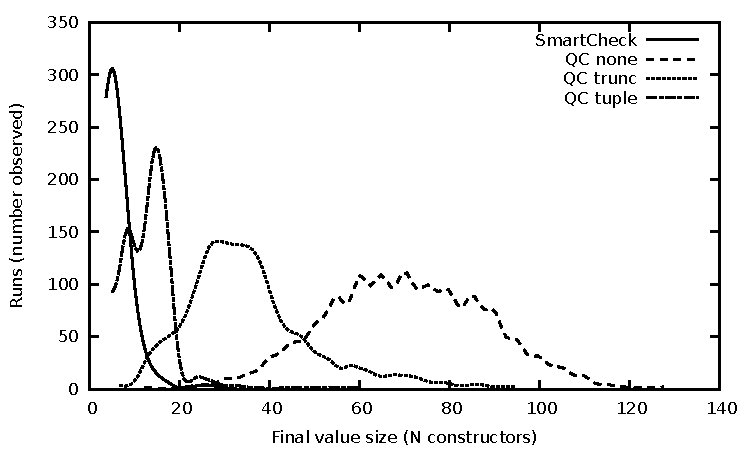
\includegraphics[scale=0.6]{Graphs/data}
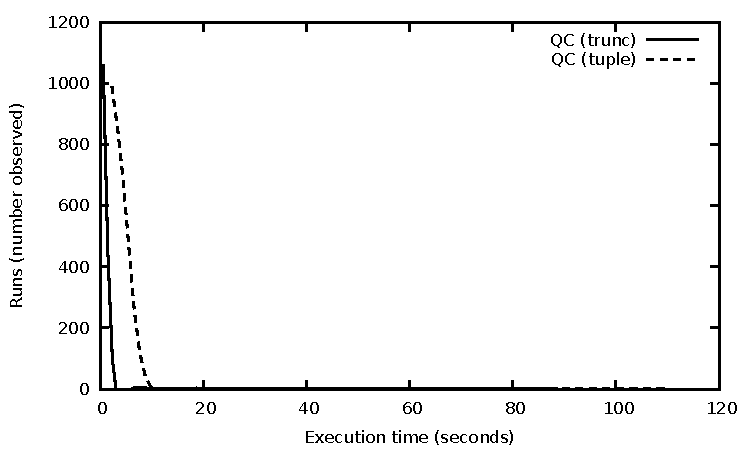
\includegraphics[scale=0.6]{Graphs/time-big}
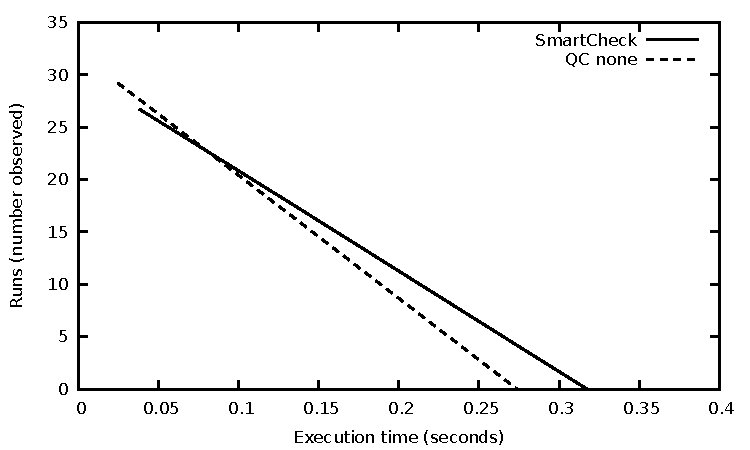
\includegraphics[scale=0.6]{Graphs/time-small}
  \caption{Results for 2000 tests of the program in Figure~\ref{fig:initial}.}
  \label{fig:graphs}
\end{figure}


\begin{table}[ht]
\footnotesize
  \begin{center}
    \begin{tabular}{|r||c|c|c|c|}
\hline
           & QC (none)  & QC (trunc) & QC (tuple) & SmartCheck\\
\hline \hline
Mean       & 0.08s, 69  & 0.53s, 35  & 2.24s, 12  & 0.10s, 7\\
\hline
Median     & 0.07s, 69  & 0.17s, 33  & 1.81s, 13  & 0.10s, 6\\
%% \hline
%% MAD        & 0.02s, 13  & 0.09s, 8   & 0.62s, 3   & 0.02s, 2\\
\hline
95\%       & 0.14s, 100 & 1.76s, 65  & 4.06s, 19  & 0.18s, 12\\
\hline
    \end{tabular}
  \end{center}
  \caption{Summarizing data for the graphs in Figure~\ref{fig:graphs}. Entries
    contain execution time (in seconds) and counterexample sizes (counting
    \ttp{N} constructors).}
  \label{table:results}
\end{table}

Motivated by these limitations of QuickCheck and SmallCheck, we developed
\emph{SmartCheck}.  SmartCheck extends QuickCheck to efficiently and generically
find small counterexamples as well as generalize them as described in the
preceding paragraph.  SmartCheck takes a counterexample produced by some
oracle---in these experiments, we use QuickCheck---and then shrinks the
counterexample.

To motivate the benefit of SmartCheck, consider the graphs in
Figure~\ref{fig:graphs} and the Table~\ref{table:results}, giving the results
for using QuickCheck and SmartCheck on the program shown in
Figure~\ref{fig:initial} (we omit SmallCheck, since as noted, it is not even
feasible for the example).  The graphs show the number of results, out of 2000
test runs, with the specified size of the final counterexample (by counting
\ttp{N} constructors) or requiring the specified execution time.  We show two
execution time graphs, since the scale of time scales differ dramatically.  In
the table, we show the mean, median, median, and the results at the 95th
percentile values.  (The curves produced by these values are not necessarily
Gaussian, so we omit standard the deviation.)

The experiments show three approaches to shrinking with QuickCheck: no
shrinking, to provide a baseline, truncated shrinking, as described above, in
which each list is truncated to 10 elements, and tuple shrinking, also described
above.  Note that SmartCheck produces smaller counterexamples than the other
approaches, with a very small tail.  SmartCheck has a very small variance---note
the mean and median are nearly identical, meaning there are very few outliers.

More dramatic, however, are the differences
in execution time.  The execution times for SmartCheck include the initial
counterexample generation time required by QuickCheck; thus the time required by
SmartCheck to shrink a counterexample is on average just 0.2 seconds (0.10 -
0.08).  As can be seen in the graphs, SmartCheck's execution time is a linear
function (like QuickCheck, without shrinking).  Truncation and tuple shrinking
produce very long tails, with some counterexamples taking over a minute to
shrink.  SmartCheck is largely insensitive to the size of the original
counterexample provided.

In the last column are the results for SmartCheck, which includes the time
required by QuickCheck to generate the original counterexample.  The median time
required by SmartCheck to shrink is 0.02 seconds (SmartCheck's execution time
minus the execution time for QuickCheck without shrinking), and the median size
of a resulting value is six \ttp{N} constructors.

And we stress that SmartCheck achieves these results \emph{generically},
requiring no shrink definitions to be provided by the user.

\paragraph{Contributions}
This paper, and the library it describes, makes the following contributions:

\begin{itemize}

\item an efficient counterexample reduction strategy for algebraic
  data types (Section~\ref{sec:shrinking});

\item an approach to counterexample generalization, to present the user with a
  formula describing a set of counterexamples to a property
  (Section~\ref{sec:generalization});

\item an approach to generically strengthen a property with a precondition that
  characterizes an already-discovered counterexample for the purpose of finding
  new, dissimilar counterexamples (Section~\ref{sec:generalization});

\item an implementation based on generic programming that is not only more
  efficient that hand-written \ttp{shrink} instances in many cases but that
  generates the instances automatically for the user
  (Section~\ref{sec:implementation}).

%% \item More generally, this paper is the first to explore the idea of
%%   efficient, generic counterexample reduction and generalization for
%%   functional program testing.
\end{itemize}

\noindent
In Section~\ref{sec:experiments}, we discuss some of our experiences with using
SmartCheck, including checking properties from Xmonad, and related work and
concluding remarks are made in Sections~\ref{sec:related}
and~\ref{sec:conclusions}, respectively.

%% \noindent Moreover, the inability to quickly uncover understandable
%% counterexamples is a real-world problem with QuickCheck (or other functional
%% languages).  It works great when your tests pass,

%% \paragraph{Outline.}
%% The paper precedes as follows.  We define a type class and some definitions in
%% Section~\ref{sec:preliminaries} used in the remainder of the paper.  In
%% Section~\ref{sec:shrinking}, we describe SmartCheck's reduction algorithm for
%% efficiently shrinking large counterexamples.  In
%% Section~\ref{sec:generalization}, we turn our attention to the problem of
%% counterexample generalization.  Here, we present two algorithms for generalizing
%% counterexamples and constructing formulas for describing them.  We also discuss
%% a method for property strengthening to discover new counterexamples.  We
%% describe implementation-specific details in Section~\ref{sec:implementation},
%% and the results of some experiments in using our tool are presented in
%% Section~\ref{sec:experiments}.  Related work is given in
%% Section~\ref{sec:related}.  Finally, concluding remarks and future work are
%% presented in Section~\ref{sec:conclusions}.


%%%%%%%%%%%%%%%%%%%%%%%%%%%%%%%%%%%%%%%%%%%%%%%%
\section{Preliminaries}\label{sec:preliminaries}

We focus on \emph{algebraic data types}~\cite{}.  Algebraic data types are
represented as ``sums of products''.  We sometimes refer to the elements of a
sum type as a \emph{variant} that is \emph{tagged} by a constructor.  For
example, the type
%
\begin{code}
Maybe a = Just a | Nothing
\end{code}
%
\noindent
contains two variants, tagged by the constructors \ttp{Just} and \ttp{Nothing},
respectively.

To present the algorithms in the following sections, we provide some definitions
in the form of methods of a \ttp{SubTypes} type class.  SmartCheck requires
instances for data being analyzed.  In Section~\ref{sec:implementation}, we
describe how instances for the type class are derived automatically.
%
\begin{code}
type Idx    = Int
type Size   = Int
data SubVal = forall a. SubTypes a => SubVal a

class Arbitrary a => SubTypes a where
  size     :: a -> Size
  index    :: a -> Idx -> Maybe SubVal
  replace  :: a -> Idx -> SubVal -> a
  constr   :: a -> String
  constrs  :: a -> [String]
  baseType :: a -> Bool
  subVals  :: a -> Tree SubVal
\end{code}
%
\noindent
The \ttp{SubTypes} type class requires QuickCheck's \ttp{Arbitrary} as a
super-class.  \ttp{SubTypes} has the following methods:
\begin{itemize}
\item \ttp{size} returns the size of a value,
\item \ttp{index} returns a \emph{sub-value} at an breadth-first index in a
  value,
\item \ttp{replace} replaces a sub-value at a particular focus (returning the
  original value if the index is out-of-bounds),
\item \ttp{constr} returns a string representation of the constructor tagging
  the value,
\item \ttp{constrs} returns the list of all possible constructors from the
  value's type,
\item \ttp{baseType} returns whether the type of the value is an ``interesting
  type'', which generally means it is user-defined and has positive arity.
  We discuss the purpose of base types in Section~\ref{sec:base}.
\item \ttp{subVals} returns a tree of all non base-type sub-values.  A tree is a
  value with the type
%
  \begin{code}
data Tree a = Node \{ rootLabel :: a
                   , subForest :: [Tree a] \}
  \end{code}
%
\end{itemize}

\noindent
To demonstrate typical evaluations of the methods, consider a binary tree type:
%
\begin{code}
data T = L | B T T
\end{code}
%
\noindent
and the value \ttp{tree}, labeled with indexes in a breadth-first order:
%
\begin{code}
tree = B\sub{0} (B\sub{1} L\sub{3}
             (B\sub{4} L\sub{6} L\sub{8}))
          (B\sub{2} L\sub{5} L\sub{7})
\end{code}
%
\noindent
Here are example applications of \ttp{SubTypes} methods; in the following, we
show the indexes with respect to the value \ttp{tree}:
%
\begin{code}
size tree = 9

index tree 4  = (Just . SubVal) (B\sub{4} L\sub{6} L\sub{8})
index tree 12 = Nothing

replace tree 2 (SubVal L) =
  B\sub{0} (B\sub{1} L\sub{3}
        (B\sub{4} L\sub{6} L\sub{8}))
     L

constr  tree = ["B"]
constrs tree = ["B", "L"]
constrs L    = ["B", "L"]

baseType (3 :: Int) = True
baseType tree       = False
baseType L          = False

subVals (B (B L\sub{0} L\sub{1}) L\sub{2}) =
  Tree (B L\sub{0} L\sub{1}) [Tree L\sub{0} [], Tree L\sub{1} []]
       (Tree L\sub{1} [])
\end{code}
%
\noindent
The \ttp{SubVal} type is an existential data type, used as a generic container
for sub-values from a counterexample.  We will sometimes refer to the unwrapped
value returned by \ttp{index a i} as the \emph{$i$th sub-value of $a$}, so for
example, (\ttp{B\sub{4} L\sub{6} L\sub{8}}) is the 4th sub-value of \ttp{tree}.
An invariant of \ttp{index} is that for any value \ttp{a}, and for the smallest
$i \geq 0$ such that
%
\begin{code}
index a i == Nothing
\end{code}
%
\noindent
then for all $0 \leq j < i$,
%
\begin{code}
index a j /= Nothing
\end{code}
\noindent
We use this invariant as a termination case in recursive algorithms over the
sub-values of a value.

In our implementation, \ttp{constr} and \ttp{constrs} depends on GHC
Generics~\cite{generics}, which we describe in Section~\ref{sec:implementation}.
For simplicity, we omit here Generics-specific super-class constraints on the
\ttp{SubTypes} class.  Moreover, our presentation simplifies the implementation
(Section~\ref{sec:implementation}) somewhat to improve the presentation.

%% Finally, \ttp{baseType} is true for our tree type but false for a
%% structureless type, such as \ttp{Int}.

% ------------------------------------------------------------------------------

\section{Shrinking Data}\label{sec:shrinking}
In this section, we describe how to efficiently shrink data values.  Before we
begin, recall the basic idea behind the \ttp{shrink} method of the
\ttp{Arbitrary} class: generate a list of values, each of which is smaller than
the current counterexample.  Each of the new values generated typically bears no
relationship to the original counterexample other than being smaller.

Consider the problem of finding a small counterexample as a graph search
problem.  The set of vertexes are all possible well-typed values.  There is an
edge from vertex $v$ to $v'$ if $v'$ is smaller than $v$ by some measure.  The
goal is to traverse the graph, starting from a counterexample, to find a vertex
from the set of smallest counterexamples in the graph.

The approach taken by \ttp{shrink} is the most naive graph search algorithm: it
simply generates a random set of potential vertexes to check in the graph.
However, it does not exploit that the original counterexample \ttp{cex} is
already in a neighborhood of other likely counterexamples.  So rather than
choose random vertexes, it may be more efficient to test other values that are
closely related to \ttp{cex}.  By restricting the search to \ttp{cex}'s
neighborhood, a smaller counterexample might be missed, and only a local minimum
is returned.  However, with a large set of values, finding a global minimum by
random sampling vertexes in the graph is possible but too inefficient, as we saw
from the example in the introduction.

\subsection{Reduction Algorithm Overview}\label{sec:reduct}
The algorithm we present for efficiently searching for new counterexamples is an
instance of greedy breadth-first search over a tree structures, representing a
value.  At each node, during the traversal, we generate arbitrary
\emph{structurally} smaller sub-values and build a new value from that, leaving
the remainder of the tree unchanged.  Intuitively, by a \emph{structurally
  smaller value}, we mean one with fewer constructors.  We continue until we
reach a fixed-point.


\begin{figure}[ht]
  \lstset{caption={}
%         ,xleftmargin=5ex,firstnumber=0,numbers=left
         }
  \begin{code}
getSize :: SubVal -> Size
getSize (SubVal a) = size a

newVals :: Size -> Int -> SubVal -> IO [SubVal]
newVals sz tries (SubVal a) =
  replicateM tries s where
  s  = liftM SubVal (sizedArbitrary sz a)

reduce :: SubTypes a
  => ScArgs -> (a -> Property) -> a -> IO a
reduce args prop cex = reduce' 1
  where
  reduce' idx
    | Just v <- index cex idx
    = do vs <- newVals (getSize v)
                 (scMaxReduce args) v
         maybe (reduce' (idx+1)) (reduce args prop)
               (test cex idx vs prop)
    | otherwise = return cex

test :: SubTypes a => a -> Idx -> [SubVal]
     -> (a -> Property) -> Maybe a
test cex idx vs prop = go vs
  where
  go []      = Nothing
  go (v:vs') =
    let cex' = replace cex idx v in
    if pass prop cex' then go vs'
      else Just cex'
  \end{code}
  \caption{Counterexample reduction algorithm.\label{fig:reduction}}
\end{figure}

Figure~\ref{fig:reduction} shows the reduction algorithm.  The function
\ttp{reduce} takes flags to customize the algorithm's behavior, a
counterexample \ttp{cex}, and the property \ttp{prop}.  At the beginning of
execution, we assume that a counterexample has been obtained somehow; our
implementation relies on QuickCheck as a ``front-end'' to generate a
counterexample that the algorithm automatically shrinks.  The reduction begins
at the first proper sub-value of \ttp{cex}; call it \ttp{v}.  When the index
\ttp{idx} becomes out-of-bounds and returns \ttp{Nothing}, the algorithm
terminates.  Otherwise, a list of new random values are generated.
%
\begin{code}
sizedArbitrary :: SubTypes a => a -> IO a
\end{code}
%
\noindent
generates a new value \ttp{v'} having the same type as \ttp{v} and that is
strictly smaller (with respect to the \ttp{size} method) than \ttp{v}.  Just
like QuickCheck's \ttp{arbitrary} method, \ttp{sizedArbitrary} generates
successfully larger counterexamples when generating new values with which to
replace a sub-value.

The flag \ttp{scMaxReduce} is the maximum number of tries to discover a new
counterexample by replacing \ttp{v} in \ttp{cex} and testing it.  The result of
\ttp{pass prop cex'} for
%
\begin{code}
pass :: (a -> Property) -> a -> Bool
\end{code}
%
\noindent
holds if \ttp{cex'} satisfies the property \ttp{prop}.  The property may be a
conditional, in which case the value must pass the precondition as well as the
consequent for \ttp{pass} to return \ttp{True}.  If no failure is found, we move
to the next sub-value of \ttp{cex} and continue.  However, if a new smaller
counterexample \ttp{cex'} is found, we start a new breadth-first traversal of
\ttp{cex'}, attempting to shrink it further.

The algorithm is guaranteed to terminate: intuitively, the measure for the
function is that either the index increases or the size of the counterexample
being evaluated decreases.  The algorithm's complexity is
$\mathcal{O}(n^2)$, where $n$ is the number of constructors in the
counterexample, assuming that generating new sub-values and testing them is done
in constant time.

\subsection{Reduction Algorithm Details}
Having describe the reduction algorithm, there are two important details about
its design we describe below.

\subsubsection{Variant Counterexample Hypothesis}
A motivation for the design of the reduction algorithm is something we cal the
\emph{variant counterexample hypothesis}.  Recall that the algorithm begins at
the \emph{first} sub-value of the counterexample rather than the 0th sub-value.
The 0th sub-value of \ttp{cex} is \ttp{cex} itself.  No invariant of the
algorithm would be violated by beginning with the 0th sub-value, and in
particular, the algorithm would still terminate.  However, we begin with a
strict sub-value because of the hypothesis.  The hypothesis is that in the
search space of possible values from a given type \ttp{T}, starting with a
particular counterexample \ttp{cex}, we are more likely to find other
counterexamples from the same variant as \ttp{cex}.  For example, consider a
property about unintended variable capture over a language's parse tree
represented by a sum type with constructors for module imports, function
definitions, and global-variable assignments, respectively.  A function
definition counterexample can only be reduced to smaller function definition
counterexamples, the only construct in which variable capture is possible.

%% Another way to motivate the hypothesis is that searching the space of
%% possible counterexamples by generating \emph{any} well-typed value that is
%% strictly smaller than the original counterexample is something we have seen
%% before: it is precisely the naive approach to implementing \ttp{shrink}!

%% \subsubsection{Conditional Properties}
%% A QuickCheck property may be a conditional of the form
%% %
%% \begin{code}
%% prop a = pre a ==> prop' a
%% \end{code}
%% %
%% \noindent
%% such that \ttp{prop} is true if the precondition (\ttp{pre a}) is false or
%% (\ttp{prop' a}) holds.  In practice, conditionals are used to restrict the set
%% of values tested; values that fail the precondition are discarded.  Thus, the
%% call to \ttp{pass} in the reduction algorithm only considers a potential
%% counterexample \ttp{cex} to have failed if it passes the property's precondition
%% and fails the consequent.

\subsubsection{Base Types}\label{sec:base}

The number of constructors in an algebraic data value primarily determines how
large it is.  In our experience, the size of fields that come from primitive
types, like \ttp{Int} or \ttp{Char}, have less of a role in understanding a
counterexample, so in general, we want to prevent our reduction algorithm from
spending time shrinking values from these types.

Consequently, we distinguish a class of types referred to as \emph{base types}.
If the reduction algorithm encounters a base type, it is ignored.  By default,
this includes numeric types (e.g., \ttp{Int}, \ttp{Word}, \ttp{Float}, etc.,
\ttp{Bool}, and \ttp{Char}.  We also treat recursive container types like lists
specially: lists of base types are considered to be base types themselves.  This
prevents the algorithm from analyzing, for example, strings.  A list of a
non-base-types is shrunk by the algorithm.

By providing custom instances, the user can declare any substructure in a data
type to be a base type.  Doing so effectively treats values from that type as
``black boxes'' for SmartCheck.  Doing so can help make SmartCheck more
efficient if the user knows that some portion of the structure cannot be shrunk
or is irrelevant to the property.

\subsection{Reduction Algorithm Optimizations}
The reduction algorithm description above omits some details and optimizations
we describe here.

\subsubsection{Sub-value Counterexample Hypothesis}\label{sec:subval}
Sometimes, a counterexample fails a property due to a sub-value nested deep
inside the counterexample.  The rest of the value is irrelevant.  We call this
the \emph{sub-value counterexample hypothesis.}  Thus, one way to efficiently
search the space of potential counterexamples is to test a counterexample's
(well-typed) sub-values.

For example, consider a simple calculator language containing constants,
addition, and division:
%
\begin{code}
data Exp = C Int
         | Add Exp Exp
         | Div Exp Exp
\end{code}
%
\noindent
Consider a program that takes an \ttp{Exp} as an argument that throws an error
if an evaluation of an \ttp{Exp} value contains a division-by-zero.  Testing for
the occurrence of the error, we might have a counterexample like the following:
%
\medskip%
\begin{sloppypar}
\small
\noindent%
\ttp{Add (Div (C 5) (C (-12))) (Add (Add (C 2) (C 4)) (Add (C 7) (Div (Add (C 7)
  (C 3)) (Add (C (-5)) (C 5)))))}
\end{sloppypar}
\medskip%
\noindent
In the counterexample, the culprit is a buried sub-value,
%
\begin{code}
Div (Add (C 7) (C 3)) (Add (C (-5)) (C 5))
\end{code}
%
Thus, when attempting to shrink an \ttp{Exp} value, it pays to test whether a
sub-value itself fails the property.

%% and consider an interpreter for the language that returns \ttp{Nothing} if
%% division-by-zero is encountered and (\ttp{Just x}), where \ttp{x} is the result
%% of the computation, otherwise:
%% %
%% \begin{code}
%% eval :: Exp -> Maybe Int
%% eval (C i) = Just i
%% eval (Add e0 e1) =
%%   liftM2 (+) (eval e0) (eval e1)
%% eval (Div e0 e1) =
%%   let e = eval e1 in
%%   if e == Just 0 then Nothing
%%     else liftM2 div (eval e0) e
%% \end{code}
%% %
%% \noindent
%% Suppose we restrict the set of programs with the following predicate:
%% %
%% \begin{code}
%% divSubTerms :: Exp -> Bool
%% divSubTerms (C _)         = True
%% divSubTerms (Div _ (C 0)) = False
%% divSubTerms (Add e0 e1)   =    divSubTerms e0
%%                             && divSubTerms e1
%% divSubTerms (Div e0 e1)   =    divSubTerms e0
%%                             && divSubTerms e1
%% \end{code}
%% %
%% and then test the property
%% %
%% \begin{code}
%% prop_div e = divSubTerms e ==> eval e /= Nothing
%% \end{code}
%% %
%% \noindent
%% The property \ttp{prop\_div} turns out to be false; for example,
%% %
%% \begin{code}
%% Div (C 1) (Div (C 0) (C 1))
%% \end{code}
%% %
%% \noindent
%% is a counterexample.  In the predicate case
%% %
%% \begin{code}
%% divSubTerms (Div _ (C 0)) = False
%% \end{code}
%% %
%% \noindent
%% we forgot to recur on the divisor.

%% %% \begin{figure}[ht!]
%% %%   \caption{Typical counterexample from QuickCheck with no user-defined
%% %%     \ttp{shrink} function.}
%% %%   \label{fig:div-cex}
%% %% \end{figure}

%% A typical counterexample returned by QuickCheck, with a \ttp{shrink} function
%% implemented, is as follows:%
%% %
%% \medskip


%% \begin{sloppypar}
%% %\makebox[\textwidth]{
%% \noindent%
%% \ttp{Div (Add (Div (Div (C (-12)) (C 22)) (Add (C 10) (C (-5)))) (Div (Add (C
%%   30) (C 12)) (C (-18)))) (Div (Div (C (-20)) (C 32)) (Div (C 10) (C (-8))))}
%% \end{sloppypar}
%% \medskip%

%% \noindent
%% It turns out that the culprit is the sub-value
%% %
%% \begin{code}
%% Div (Div (C (-20)) (C 32)) (Div (C 10) (C (-8)))
%% \end{code}
%% %
%% \noindent
%% Thus, while analyzing the counterexample above

\begin{figure}
\begin{code}
reduceOpt :: forall a . SubTypes a
  => ScArgs -> (a -> Property) -> a -> IO a
reduceOpt args prop cex = reduce' 1
  where
  reduce' idx
    | Just v <- index cex idx
    = maybe (test' v idx) (reduceOpt args prop)
            (testHole v)
    | otherwise = return cex

  test' v idx = do
    vs <- newVals (getSize v) (scMaxReduce args) v
    maybe (reduce' (idx+1)) (reduceOpt args prop)
          (test cex idx vs prop)

  testHole (SubVal a) = do
    a' <- cast a :: Maybe a
    if pass prop a' then Nothing else Just a'
\end{code}
  \caption{Reduction algorithm with the sub-value counterexample optimization.}
  \label{fig:reduce0}
\end{figure}

Generalizing the scenario, during the reduction algorithm's breadth-first
search through a counterexample \ttp{cex}'s sub-values, we may happen upon a
sub-value \ttp{cex'} that has the same type as \ttp{cex} and fails the property
(while passing any preconditions).  In this case, we can return \ttp{cex'}
directly, and rerun the reduction algorithm on \ttp{cex'}.  In
Figure~\ref{fig:reduce0}, we show an updated reduction algorithm, \ttp{reduceOpt},
that implements this optimization.  The function \ttp{testHole} tests the
current sub-value and if it fails the property, the function tests the sub-value
directly.


\subsubsection{Bounding Counterexample Exploration}

SmartCheck's implementation contains flags to allow the user to customize its
behavior.  Three flags that are relevant to the reduction algorithm are the
following:
%
\begin{code}
scMaxReduce :: Int
scMaxSize   :: Int
scMaxDepth  :: Maybe Int
\end{code}
%
\noindent
The \ttp{scMaxReduce} flag controls the number of values generated by the
reduction algorithm for each sub-value analyzed.  \ttp{scMaxSize} controls the
maximum size of values generated to replace sub-values by the reduction
algorithm.  Thus, new sub-values must be strictly smaller than the minimum of
\ttp{scMaxSize} and the size of the sub-value being replaced.  Finally,
\ttp{scMaxDepth} determines the maximum depth in the counterexample the
reduction algorithm should analyze.  A value of \ttp{Nothing} means that the
counterexample should be exhaustively reduced, as the algorithm is presented in
Figure~\ref{fig:reduction}.  For example, the depth of a list is determined by
its length, and the depth of the binary tree defined in Section~\ref{sec:reduct}
is determined by the function \ttp{depth}:
%
\begin{code}
depth L         = 0
depth (B t0 t1) = 1 + max (depth t0) (depth t1)
\end{code}
%
\noindent
Of the flags, \ttp{scMaxDepth} is the most important for controlling
efficiency, particularly for large product types with significant ``fan out''.
The number of sub-values of a value product type can grow exponentially with
respect to the depth.  Furthermore, note that as the reduction algorithm
descends further, there is less chance to reduce the size of the value overall,
since smaller and smaller sub-values are replaced.

\section{Counterexample Generalization}\label{sec:generalization}

Small counterexamples make debugging easier, but they are just half the battle.
To go from a specific counterexample to the required fix in a program, the
programmer must have a flash of insight in which she generalizes the
counterexample to a set of counterexamples for which the program and property
fails.  The generalization step is an important yet under-appreciated step in
the debugging process.  A characterizing formula reduces the noise in favor of
the signal by abstracting away portions of large counterexample that are
irrelevant to why it violates the property.

The characterization of counterexamples that most helps the programmer should
strike a middle ground.  A single counterexample is too specific.  On the other
hand, the property itself is a formula that over-approximates the failing
inputs.  We describe two kinds of formula that fall between these two extremes.

\subsection{Universal Sub-Value Generalization}\label{sec:universal}
Recall from the introduction the quantified formula
%
\begin{code}
forall x . T x [N (-20000)] [N (-20000)] [] []
\end{code}
%
\noindent
characterizing a set of counterexamples.  Another example using the calculator
language from Section~\ref{sec:subval} is to generalize a counterexample like
%
\begin{code}
Div (Add (C 7) (C 3)) (Add (C (-5)) (C 5))
\end{code}
%
\noindent
by
%
\begin{code}
forall x . Div x (Add (C (-5)) (C 5))
\end{code}
%
\noindent
since any dividend results in divide-by-zero.  Not only do the generalizations
assist the programmer's insight, but they reduce the sheer size of the
counterexample.  We call the kind of formula just shown \emph{universal
  sub-value generalization} and is implemented in SmartCheck.

An extrapolation algorithm performs universal sub-value generalization.  The
basic idea is as follows: for a counterexample \ttp{cex} and a property
\ttp{prop}, a breadth-first search over the sub-values of the \ttp{cex} is
performed.  For each sub-value, the algorithm generates new sub-values, replaces
them in \ttp{cex} to create a list of new potential counterexamples.  If enough
new counterexamples non-trivially fail \ttp{prop} (i.e., fail the property's
consequent but satisfy its antecendent), then we extrapolate, claiming that for
\emph{any} new value replacing that sub-value in \ttp{cex}, the property will
fail.

\begin{figure}
  \begin{code}
subTrees :: SubTypes a => a -> Idx -> [Idx] -> Bool
subTrees cex idx = any (subTree cex idx)

extrapolate :: SubTypes a
  => ScArgs -> a -> (a -> Property) -> IO [Idx]
extrapolate args cex prop = extrapolate' 1 []
  where
  extrapolate' idx idxs
    | subTrees cex idx idxs
    = extrapolate' (idx+1) idxs
    | Just v <- index cex idx = mkNewVals v
    | otherwise = return idxs
    where
    mkNewVals v = do
      vs <- newVals (scMaxSize args)
                    (scMaxForall args) v
      extrapolate' (idx+1)
        (if allFail args cex idx vs prop
           then idx:idxs else idxs)

allFail :: SubTypes a => ScArgs -> a -> Idx
  -> [SubVal] -> (a -> Property) -> Bool
allFail args cex idx vs prop =
  length res >= scMinForall args && and res
  where
  res  = mapMaybe go vs
  go   = fail prop . replace cex idx
  \end{code}
  \caption{Universal sub-value generation algorithm.}
  \label{fig:universal}
\end{figure}

\todo{explain scMaxForall}

The extrapolation algorithm is shown in Figure~\ref{fig:universal}.  The
algorithm is similar to the reduction algorithm in Figure~\ref{fig:reduction},
and in the implementation, the algorithms are generalized and combined.  The
function \ttp{extrapolate} returns a list of indexes to be generalized in the
original counterexample.  In the recursive function \ttp{extrapolate'}, there is
a function guard in which a call
%
\begin{code}
subTree cex idx0 idx1
\end{code}
%
\noindent
where \ttp{subTree} has the type
%
\begin{code}
subTree :: SubTypes a => a -> Idx -> Idx -> Bool
\end{code}
%
\noindent
is true if in \ttp{cex}, the value at index \ttp{idx0}, is a child of index
\ttp{idx1}, in a tree representation of \ttp{cex} (i.e., \ttp{subVals cex}).  This
prevents the algorithm from trying to generalize sub-values that are abstracted
away already since their parents have been generalized.

New sub-values are generated by \ttp{newVals}, shown in
Figure~\ref{fig:reduction}.  Here, we bound the size of values to generate by
the flag \ttp{scMaxSize}, which is independent of the size of the particular
sub-value.

The function \ttp{allFail} takes a counterexample \ttp{cex}, an index into
\ttp{cex}, a list of new sub-values, and a property.  It returns true if enough
new values pass the property's precondition and fail the property.  The function
%
\begin{code}
fail :: (a -> Property) -> a -> Maybe Bool
\end{code}
%
\noindent
is roughly the dual of \ttp{pass} in the reduction algorithm: (\ttp{fail
  prop cex}) returns (\ttp{Just True}) if \ttp{cex} passes \ttp{prop}'s
precondition but fails the property; (\ttp{Just False}) if \ttp{cex}
non-trivially satisfies \ttp{prop}, and \ttp{Nothing} if \ttp{cex} fails
\ttp{prop}'s precondition.  The flag \ttp{scMinForall} is the minimum number
of \ttp{Just False} results required from \ttp{fail} to extrapolate from failed
tests to a universal claim.

The extrapolation algorithm is unsound insofar as it extrapolations from a set
of counterexamples to a universal claim, similar to QuickSpec~\cite{qs}.  By
tuning the parameters, the risk of an unsound generalization is reduced.

The algorithm's complexity is $\mathcal{O}(n)$, where $n$ is the number of
constructors in the counterexample.  Again, we assume that the cost for each
generating random values and testing them at each index is constant.


\subsection{Existential Sub-Value Generalization}

Sum types denote choice in a data type.  Sometimes, a property over a sum type
fails because there is a bug for some of the variants but not others.  For
example, recall the calculator language from Section~\ref{sec:subval}.  The
property \ttp{prop\_div} fails only for values that contain a variant tagged
with the \ttp{Div} constructor.  Recall again the generalized counterexample
from Section~\ref{sec:generalization}:
%
\begin{code}
forall x . Div x (Add (C (-5)) (C 5))
\end{code}
%
\noindent
Because the divisor does not generalize, we know there is something special
about it that causes failure.  But we might wonder if there is something special
about variants tagged by the \ttp{Add} constructor, or might we finding failing
sub-values with the other variants.

We therefore introduce another kind of generalization we call \emph{existential
  sub-value generalization}.  In this generalization, if there a counterexample
containing every possible variant as a sub-value, then we abstract it.  For
example, the following all characterize counterexamples:
%
\begin{code}
Div (C 7) (Add (C (-5)) (C 5))
Div (Add (C 3) (C 2)) (C 0)
Div (C (-2)) (Div (C 0) (C 1))
\end{code}
%
\noindent
Because there are only three variants in the type, we have found counterexamples
built from each of them in the divisor.  We therefore can claim the following
formula holds:
%
\begin{code}
forall values x .
  forall constructors C .
    there exist arguments \(\stackrel{\rightarrow}{y}\) .
      such that Div x (C\(\stackrel{\rightarrow}{y}\))
\end{code}
%
\noindent
We therefore present an existential sub-value generalization algorithm that
performs constructor generalization.  Like with the other algorithms, this
algorithm also performs a breadth-first search over a counterexample.

\begin{figure}
  \begin{code}
subConstr :: SubVal -> String
subConstr (SubVal a) = constr a

subConstrs :: SubVal -> [String]
subConstrs (SubVal a) = constrs a

sumTest :: SubTypes a => ScArgs -> a
  -> (a -> Property) -> [Idx] -> IO [Idx]
sumTest args cex prop exIdxs = sumTest' 1 []
  where
  sumTest' idx idxs
    | subTrees cex idx (exIdxs ++ idxs)
    = sumTest' (idx+1) idxs
    | Just v <- index cex idx = fromSumTest v
    | otherwise = return idxs
    where
    fromSumTest v = do
      vs <- newVals (scMaxSize args)
              (scMaxExists args) v
      sumTest' (idx+1)
        (if constrFail cex idx vs prop
           (subConstr v) (subConstrs v)
           then idx:idxs else idxs)

constrFail :: SubTypes a => a -> Idx -> [SubVal]
  -> (a -> Property) -> String -> [String] -> Bool
constrFail cex idx vs prop con allCons =
  constrFail' [con] vs
  where
  constrFail' cons vs'
    | length cons == length allCons = True
    | null vs'                      = False
    | go v == Just True
    = constrFail' (c:cons) (tail vs')
    | otherwise
    = constrFail' cons (tail vs')
    where
    v  = head vs'
    c  = subConstr v
    go = fail prop' . replace cex idx
    prop' a = c `notElem` cons ==> prop a
  \end{code}
  \caption{Universal sub-value generation algorithm.}
  \label{fig:constrs}
\end{figure}

We show the algorithm in Figure~\ref{fig:constrs}.  The function \ttp{sumTest}
takes a set of flags, a counterexample, a property, and a list of indexes that
have already been generalized---perhaps by the extrapolation algorithm in
Figure~\ref{fig:universal}.  The list of course may be empty if no sub-values
have been previously extrapolated.  In a call to \ttp{subTrees}, discussed in
Section~\ref{sec:universal}, the guard prevents constructor generalization if
the current index is a sub-value of a previously generalized value.  Otherwise,
a list of well-typed new values are generated by a call to \ttp{newVals}, as
shown in Figure~\ref{fig:reduction}.  In the arguments to \ttp{newVals}, we
bound the size of values generated with \ttp{scMaxSize} as before, and bound the
number of values generated with the flag \ttp{scMaxExists}.  Because values are
randomly generated, for ``wide'' sum-types (i.e., with a large number of
constructors), \ttp{scMaxExists} should be large enough to ensure with high
probability that each variant is generated.

The function \ttp{constrFail} returns true if we replace the sub-value at index
\ttp{idx} in counterexample \ttp{cex} with every possible variant given the type
and construct a counterexample to the property.  There are three guards to the
recursive function \ttp{constrFail'}: the first guard holds if the list of
constructors tagging variants in which a counterexample is found is equal in
size to the list of all possible constructors for the type.  The second guard
tests whether the set of test values is null; if so (and if the first guard
fails), then we have exhausted test values before finding all possible failing
variants.  Third, for a specific sub-value \ttp{v}, we test whether it fails the
property.  If so, we add its constructor to the list of constructors.  Note in
the definition of \ttp{prop'}, we add an additional precondition that the
current constructor is not an element of constructors already seen.  Thus,
(\ttp{go v}) returns (\ttp{Just True}) if (\ttp{replace cex idx v}) passes this
precondition (and any other preconditions of \ttp{prop}), but fails the
property.

Unlike universal sub-value generalization, existential sub-value generalization
is sound.  The existential claim is only that for each variant, there exists at
least one counterexample, so inductive reasoning is not required.

This algorithm's complexity is also $\mathcal{O}(n)$, where $n$ is the number of
constructors in the counterexample.

\subsection{Automated Precondition Strengthening}\label{sec:precondition}
The extrapolation algorithm generalizes a counterexample, but in the
``neighborhood'' of he original counterexample.  In particular, all
generalizations are from the same variant as the original counterexample.  To
help the programmer in the generalization step, we would also like a way to test
the property again, ensuring we get counterexamples (if they exist) outside of
the neighborhood of the original one.

\begin{figure}[ht!]
  \begin{center}
    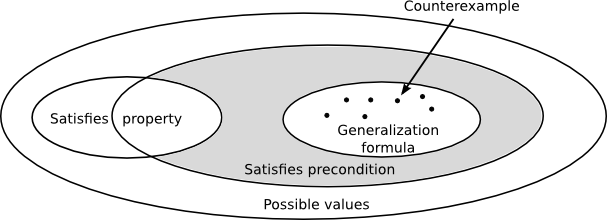
\includegraphics[scale=0.49]{Figs/cex-gen}
   \end{center}
  \caption{Counterexample generalization.}
  \label{fig:cex-gen}
\end{figure}

Figure~\ref{fig:cex-gen} illustrates the situation in which we have some values
and a property in the case that some values fail the property of the form
(\ttp{pre ==> prop}).  Our goal is to find additional counterexamples in the
shaded region, in which \ttp{pre} is satisfied, \ttp{prop} is not satisfied, and
the counterexample is not already characterized by a universal sub-value
generalization formula.  Iterating, we increasingly cover the shaded region
with new formulas until no more uncovered counterexamples exist or the testing
tool fails to find new counterexamples.

\begin{figure}
  \begin{code}
matchesShapes :: SubTypes a
  => a -> [(a,[Idx])] -> Bool
matchesShapes d = any (matchesShape d)

matchesShape :: SubTypes a
  => a -> (a, [Idx]) -> Bool
matchesShape a (b, idxs)
  | constr a /= constr b = False
  | Just a' <- aRepl
  = let x = subForest (subVals a') in
    let y = subForest (subVals b)  in
    all foldEqConstrs (zip x y)
  | otherwise = False
  where
  updateA idx d =
    fmap (replace d idx) (index b idx)
  aRepl = foldl go (Just a) idxs where
    go ma idx | Just x <- ma = updateA idx x
              | otherwise    = Nothing
  foldEqConstrs ( Node (SubVal l0) sts0
                , Node (SubVal l1) sts1 )
    | constr l0 == constr l1 =
      all foldEqConstrs (zip sts0 sts1)
    | otherwise              = False
  \end{code}
  \caption{Shape matching algorithm.}
  \label{fig:matches}
\end{figure}

Figure~\ref{fig:matches} show the shape-matching algorithm used for precondition
strengthening.  The function takes a candidate counterexample and a list of
previous counterexamples, together with the indexes at which they have been
generalized.  The basic idea of the algorithm is to determine whether two values
have the same ``shape''.  Intuitively, we consider two values to have the same
shape if in their respective tree representations, their constructors at each
node in the tree match, ignoring all base types (Section~\ref{sec:base}).
That is, intuitively, for values \ttp{a} and \ttp{b},
%
\begin{code}
subVals a == subVals b
\end{code}
%
\noindent
Furthermore, indexes that have been universally generalized (and all their
children) match any value, since a universally generalized index indicates that
counterexamples have been found for any possible constructor.  In our
implementation, we also consider existentially generalized indexes to match any
value.  Doing so is a design choice that is more aggressive about covering the
space of counterexamples at the risk of omitting some.

To understand the shape matching algorithm, consider a few values of type
\ttp{Exp}, defined in Section~\ref{sec:subval}:
%
\begin{code}
e0 = Div (C 1) (C 2)
e1 = Div (C 1) (C 3)
e2 = Div (Add (C 1) (C 2)) (C 7)
e3 = Div (Div (C 8) (C 2)) (C 7)
\end{code}
%
\noindent
Then the following hold:
%
\begin{code}
matchesShape e0 (e1, [])  == True
matchesShape e1 (e2, [])  == False
matchesShape e1 (e2, [0]) == True
matchesShape e3 (e2, [0]) == True
\end{code}
%
The first equation holds because we ignore base types.  The second equation
fails because at index 0, \ttp{e1} contains the constructor \ttp{C} and \ttp{e2}
contains the constructor \ttp{Add}.  However, index 0 has been generalized, then
we ignore the sub-value at index 0, and they match (the third equation).
The same reasoning holds for the fourth equation.


\section{Implementation and Usage}\label{sec:implementation}

The implementation of SmartCheck is written in Haskell and is designed to test
Haskell programs.  The source code is licensed BSD3 and is freely
available.\footnote{\url{https://github.com/leepike/SmartCheck.git}}

SmartCheck generically operates over arbitrary algebraic data and so uses a
generics library to encode generic traversals.  Specifically, SmartCheck uses
``GHC Generics'', a recently-developed generics library for
Haskell~\cite{generics}.  The generics library allows algebraic data types to
automatically derive the type class \ttp{SubTypes} presented in
Section~\ref{sec:preliminaries}.  One limitation with GHC Generics is that it
does not (currently) support generalized algebraic data types~\cite{gadts}.

The data type to be tested must derive the \ttp{Read}, \ttp{Show},
\ttp{Typeable}, and \ttp{Generic} type classes.  Deriving \ttp{Typeable} and
\ttp{Generic} require using the GHC language extensions \ttp{DeriveDataTypeable}
and \ttp{DeriveGeneric}, respectively.  \ttp{Typeable} is used for dynamic
typing in defining the \ttp{replace} method of \ttp{SubTypes} since it is
unknown at compile-time whether the value to be replaced and replacing value
have the same types.

Then, the user simply declares, for a data type \ttp{D},
%
\begin{code}
instance Subtypes D
\end{code}
%

SmartCheck does not implement a counterexample discovery algorithm.  While any
method can be used to discover an initial counterexample, SmartCheck by default
uses QuickCheck to discover an initial counterexample.  If QuickCheck is used,
instances for \ttp{Arbitrary} must be provided.

A property may be a function taking any number of arguments, but SmartCheck only
operates on a single input during testing, which is assumed to be the first
argument to the function.  Our experience is that often a program operates over
one large structure together with smaller inputs.  While multiple inputs could
be analyzed simultaneously by SmartCheck, it is not clear how to clearly
represent multiple large counterexamples to the user---the implementation
currently prints to standard out.  (In future work, a web-based interface could help.)

A read-eval-print loop is presented to the user, allowing her to iterate shrink
and generalize counterexamples, and then generate new counterexamples after
strengthening the property's precondition as described in
Figure~\ref{sec:precondition}.

SmartCheck is executed using
%
\begin{code}
> smartCheck args prop
\end{code}
%
\noindent
where \ttp{args} are the arguments passed in, and \ttp{prop} is the property
being tested.  The arguments is a record type that includes the values described
above to control SmartCheck's behavior.

\todo{default instances for all common types, including those provided by QC}

\section{Experiments}\label{sec:experiments}

\subsection{Xmonad}
Xmonad is a popular X11 window manager written in Haskell~\cite{xmonad}.  Xmonad
is a large software project with many contributors, so consequently, a
QuickCheck test harness is included to help ensure new commits do not introduce
bugs.  At the heart of Xmonad is a \ttp{StackSet} data type that encodes the
relationship between windows, work spaces, and which window has the focus.
Xmonad contains properties to ensure the correct manipulation of
\ttp{StackSet}s.

Xmonad passes all of its QuickCheck tests, but let us see what might happen to a
new contributor if things go awry.  Suppose a developer defines an insertion
function that inserts a new focus into the \ttp{StackSet}, except she forgets to
place the value inside.  The correct insertion function from Xmonad is
%
\begin{code}
insertUp a s = if member a s then s else insert
  where
  insert = modify (Just $ Stack a [] [])
                  (\textbackslash(Stack t l r) ->
                      Just $ Stack a l (t:r)) s
\end{code}
%
\noindent
So suppose the developer forgets to cons \ttp{t} onto \ttp{r}.  Fortunately,
there are QuickCheck tests that depend on \ttp{insertUp}.  One such test is
\ttp{prop\_shift\_reversible}, which tests if the \ttp{shift} function, which
checks a property about shifting focus back and forth between windows.

With the incorrect version of \ttp{insertUp}, QuickCheck returns a wall of text
to the user, showing the fields of a \ttp{StackSet}:

\medskip%
\begin{sloppypar}
\footnotesize
\noindent%
\ttp{StackSet \{current = Screen \{workspace = Workspace \{tag = NonNegative
  \{getNonNegative = 5\}, layout = -2, stack = Just (Stack \{focus = 'I', up =
  ", down = "\})\}, screen = 5, screenDetail = 0\}, visible = [Screen
    \{workspace = Workspace \{tag = NonNegative \{getNonNegative = 0\}, layout =
    -2, stack = Just (Stack \{focus = '\char`\\161', up = \", down =
    \"\})\}, screen = 1, screenDetail = -2\},Screen \{workspace = Workspace
    \{tag = NonNegative \{getNonNegative = 2\}, layout = -2, stack = Just (Stack
    \{focus = '3', up = \", down = "\})\}, screen = 2, screenDetail =
    -1\},Screen \{workspace = Workspace \{tag = NonNegative \{getNonNegative =
    3\}, layout = -2, stack = Just (Stack \{focus = 'T', up = \", down =
    \"\})\}, screen = 3, screenDetail ) = 2\},Screen \{workspace = Workspace
    \{tag = NonNegative \{getNonNegative = 4\}, layout = -2, stack = Nothing\},
    screen = 4, screenDetail = -1\},Screen \{workspace = Workspace \{tag =
    NonNegative \{getNonNegative = 6\}, layout = -2, stack = Just (Stack \{focus
    = 'm', up = \", down = \"\})\}, screen = 6, screenDetail = 2\},Screen
    \{workspace = Workspace \{tag = NonNegative \{getNonNegative = 7\}, layout =
    -2, stack = Nothing\}, screen = 0, screenDetail = 0\}], hidden = [Workspace
    \{tag = NonNegative \{getNonNegative = 1\}, layout = -2, stack = Just (Stack
    \{focus = '\char`\\DC3', up = \", down = \"\})\},Workspace \{tag = NonNegative \{getNonNegative = 8\}, layout = -2, stack = Nothing\},Workspace \{tag = NonNegative \{getNonNegative = 9\}, layout = -2, stack = Just (Stack \{focus = '\char`\\ACK', up = \", down = \"\})\}], floating = fromList []\} }
\end{sloppypar}
\medskip%
\noindent
This is a wall of text, which provides little useful information about what went
wrong.  SmartCheck, however, takes the value and returns the following:
%
\begin{code}
Extrapolated value:
forall x0 x1 x2:
  StackSet x0 x1 x2 (fromList [])
\end{code}
%
\noindent
The programmer immediately sees that the first three fields in the record are
irrelevant,  The last field is a dictionary (i.e., an ordered map), which we
declare to be a base type, so it is not analyzed by SmartCheck.  The upshot is
that any \ttp{StackSet} fails because insertion is ill-defined.  Such an
insight, while obvious in hind-sight, can take hours to arrive at as the
programmer manually tries to write her own shrink functions or manually
deconstruct a large record.


\todo{xmonad} \todo{experiments? scale vs. broad data, linear data?}

%-------------------------------------------------------------------------------


%-------------------------------------------------------------------------------
\section{Related Work}\label{sec:related}

Counterexample reduction in general is a relatively unexplored topic, but there
has been some treatment of the topic.  Zeller and Hildebrandt describe an
application of greedy search to shrink counterexamples they call
``delta-debugging'' (DD)~\cite{dd}.  The authors apply their work shrinking HTML
inputs to crash Mozilla and shrinking C programs to trigger a bug in GCC.
Subsequent generalizations are reported by Misherghi and Su in which they
perform greedy search on tree-structured data; they call their approach
hierarchical delta-debugging (HDD)~\cite{hdd}.

HDD is most similar to SmartCheck's reduction algorithm, with an important
difference: HDD (and DD) is deterministic, so the algorithm only succeeds in
reducing the counterexample only if a new counterexample can be constructed from
the original one.  Our approach combines the speed of delta debugging with the
power of QuickCheck to \emph{randomly} discover structurally smaller
counterexamples; in short, this is the first treatment we know of that
integrates counterexample generation with counterexample reduction.
Furthermore, neither paper explores the idea of counterexample generalization.

Within the functional programming community, one of the few treatments of
generic shrinking is as a motivation for generic programming in Haskell's
``Scrap your boilerplate'' generic programming library~\cite{syb}.

Besides QuickCheck and SmallCheck, another testing framework related to
SmartCheck is the recent Haskell library Feat~\cite{feat}.  Feat provides
automated enumerations of algebraic data types in Haskell, allowing for fast
access to very large indexes.  For example, from the enumeration of
(\ttp{[Bool]})
%
\begin{code}
[[],[False],[True],[False,False],[False,True] ...
\end{code}
%
\noindent
Accessing the $10^{1000}$th element takes under $0.1$ seconds in interpreted
Haskell.  Feat combines some advantages of SmallCheck and QuickCheck, since the
user can choose to exhaustively test an enumeration up to some depth, like with
SmallCheck, or she can create a uniform distribution of test cases up to some
depth.

Feat finds small counterexamples effectively, but a limitation compared to
QuickCheck is that value generation is applicative rather than monadic.
Consequently, defining custom generators (i.e., instances for \ttp{arbitrary})
is highly constrained.  On the other hand, generators can be derived
automatically with Feat.

We have benchmarked Feat as well on the example in the introduction
(Figure~\ref{fig:initial}).  While it performs quite competitively to SmartCheck
in terms the size of counterexamples discovered: the mean and median number of
\ttp{N} constructors in the counterexamples returned by Feat are both seven.
However, Feat performs more poorly with respect to how long counterexample
discovery takes: the mean time taken by Feat is 5.60 seconds, with a long tail:
five percent of runs take over 14 seconds (the mean time taken by
SmartCheck is 0.12 seconds, and 99\% of runs take less than 0.30 seconds).

SmartCheck bears some similarity to QuickSpec, a testing-based library that
infers equational properties about programs~\cite{qs} insofar as they both
attempt to generalize counterexamples based on specific inputs.

%% \todo{avoid complexities \url{http://stackoverflow.com/questions/14006005/idiomatic-way-to-shrink-a-record-in-quickcheck}%
%% %
%% * Also check out \url{http://www.whyprogramsfail.com/}%
%% %
%% \url{http://www.haskell.org/haskellwiki/Research_papers/Testing_and_correctness}%}
%% \todo{shrink paper rehger pointed to ``Automatic isolation of compiler errors''
%%   from 1994}

%% \todo{Not relevant really: GenCheck
%%   \url{https://github.com/JacquesCarette/GenCheck}%
%% \url{http://blog.regehr.org/archives/697} --- check out C-reduce (Regehr)
%% \todo{\url{http://www.cs.utah.edu/~regehr/papers/pldi12-preprint.pdf}}
%% }

%-------------------------------------------------------------------------------
\section{Conclusions and Future Work}\label{sec:conclusions}

We have presented new approaches for generically shrinking and generalizing
counterexamples over algebraic data.  Shrinking has thus far been as much an art
as a science, requiring experience with QuickCheck and deep understanding about
the property being tested.  In many cases, SmartCheck automates the laborious
task of shrinking.

We envision a number of potential extensions and improvements to SmartCheck.
First, we have considered only the simplest kind of data, algebraic data types,
but we would like to extend these results to shrinking functions, too.  As noted
in Section~\ref{sec:implementation}, SmartCheck does not work with GADTs
currently, due to limitations with GHC Generics.

We have not profiled the performance of our implementation of SmartCheck, so
additional performance gains might be possible.  In particular, we perform
significant computations over tree-structured data, and a zipper~\cite{zipper},
which we do not currently implement, could improve performance.

Lazy SmallCheck can test partially-defined inputs by detecting the evaluation of
undefined values~\cite{sc}.  This capability is useful in shrinking, too.  For
example, the universal sub-value generalization algorithm
(Section~\ref{sec:universal}) could be extended to shortcut testing and
generalize a sub-value if it is not evaluated in testing the property.  Not only
does this shortcut the generalization phase, but it gives a proof that the
sub-value can be generalized.

SmartCheck displays (generalized) counterexamples in a form similar to default
\ttp{Show} instances or in a tree form, which can be helpful to parse the
components of the value.  Better approaches for showing large data types are
needed.

Finally, we believe there are interesting connections between counterexample
discovery and probabilistic reasoning.  Often, when a bug in a program is fixed,
the fix is not correct, or it introduces new bugs.  Such knowledge might be
useful in guiding the distribution of test cases or shrinking.

\todo{difficult to compare performance against arbitrary hand-written shrinking}
\todo{final summary}

\section*{Acknowledgements}
\todo{Thank Rehger for comments/pointing to paper.}

%% \balancecolumns

\bibliographystyle{abbrvnat}
\bibliography{paper}

\end{document}

